\newpage
\section{Diseño del Sistema}
	A continuación se muestra parte del diagrama de clases y el diagrama de
	procesos (BPM):\footnote{Se puede encontrar los diagramas completos y legibles
	en
	\href{https://www.github.com/w11ld33r/informe-practicas/tree/master/imgs}{https://www.github.com/w11ld33r/informe-practicas/tree/master/imgs}}

	\begin{figure}[H]
	    \centering
		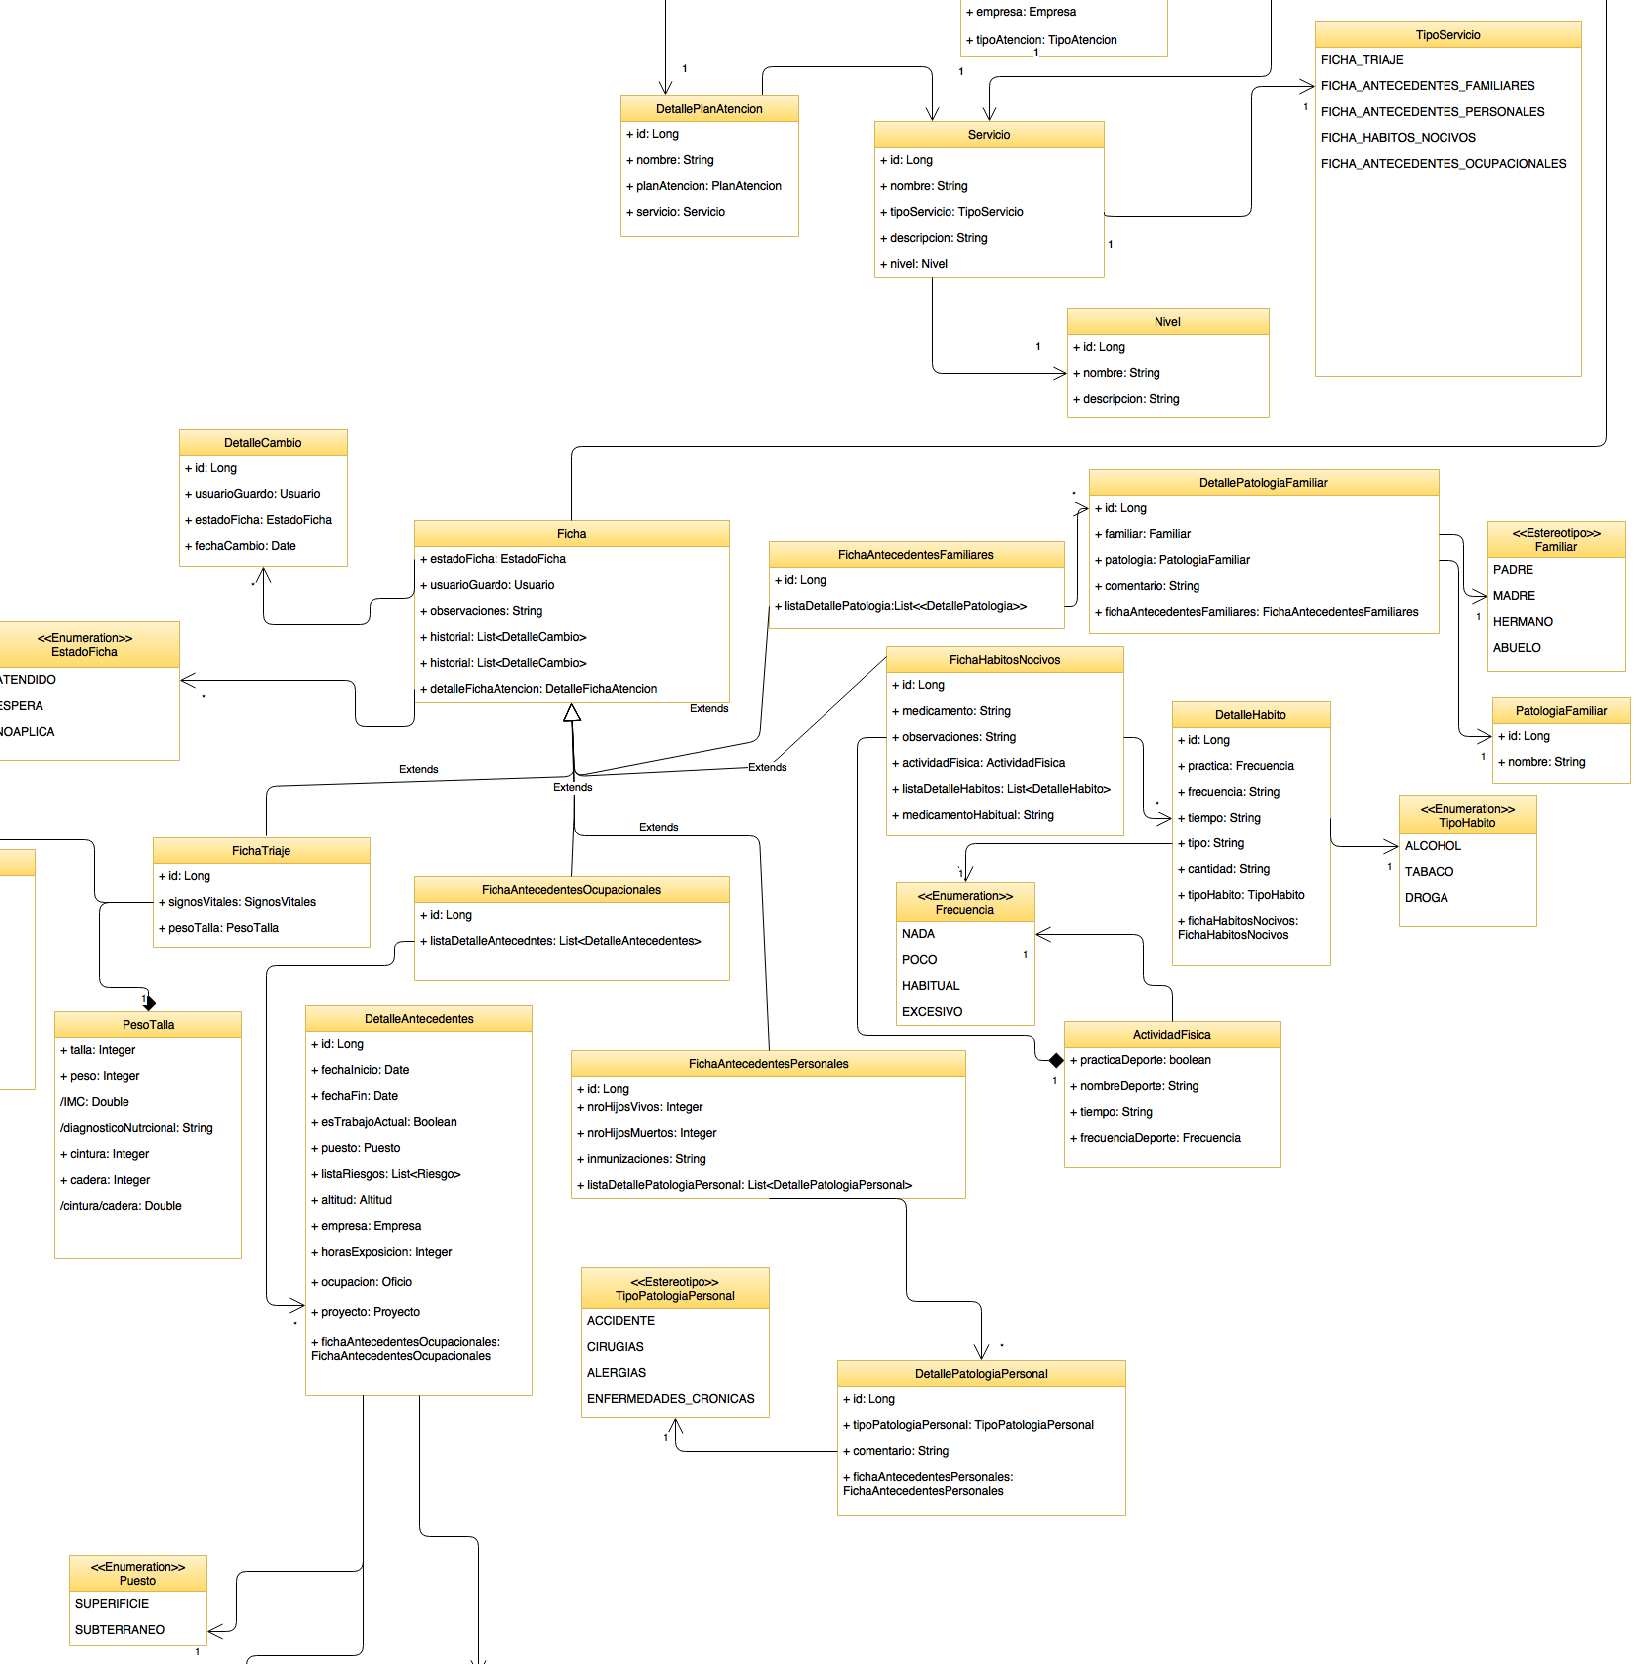
\includegraphics[width=17cm]{../imgs/disenio/DC2.png}
		\caption{DC-A Diagrama de clases}
	\end{figure}
	\begin{figure}[H]
	    \centering
		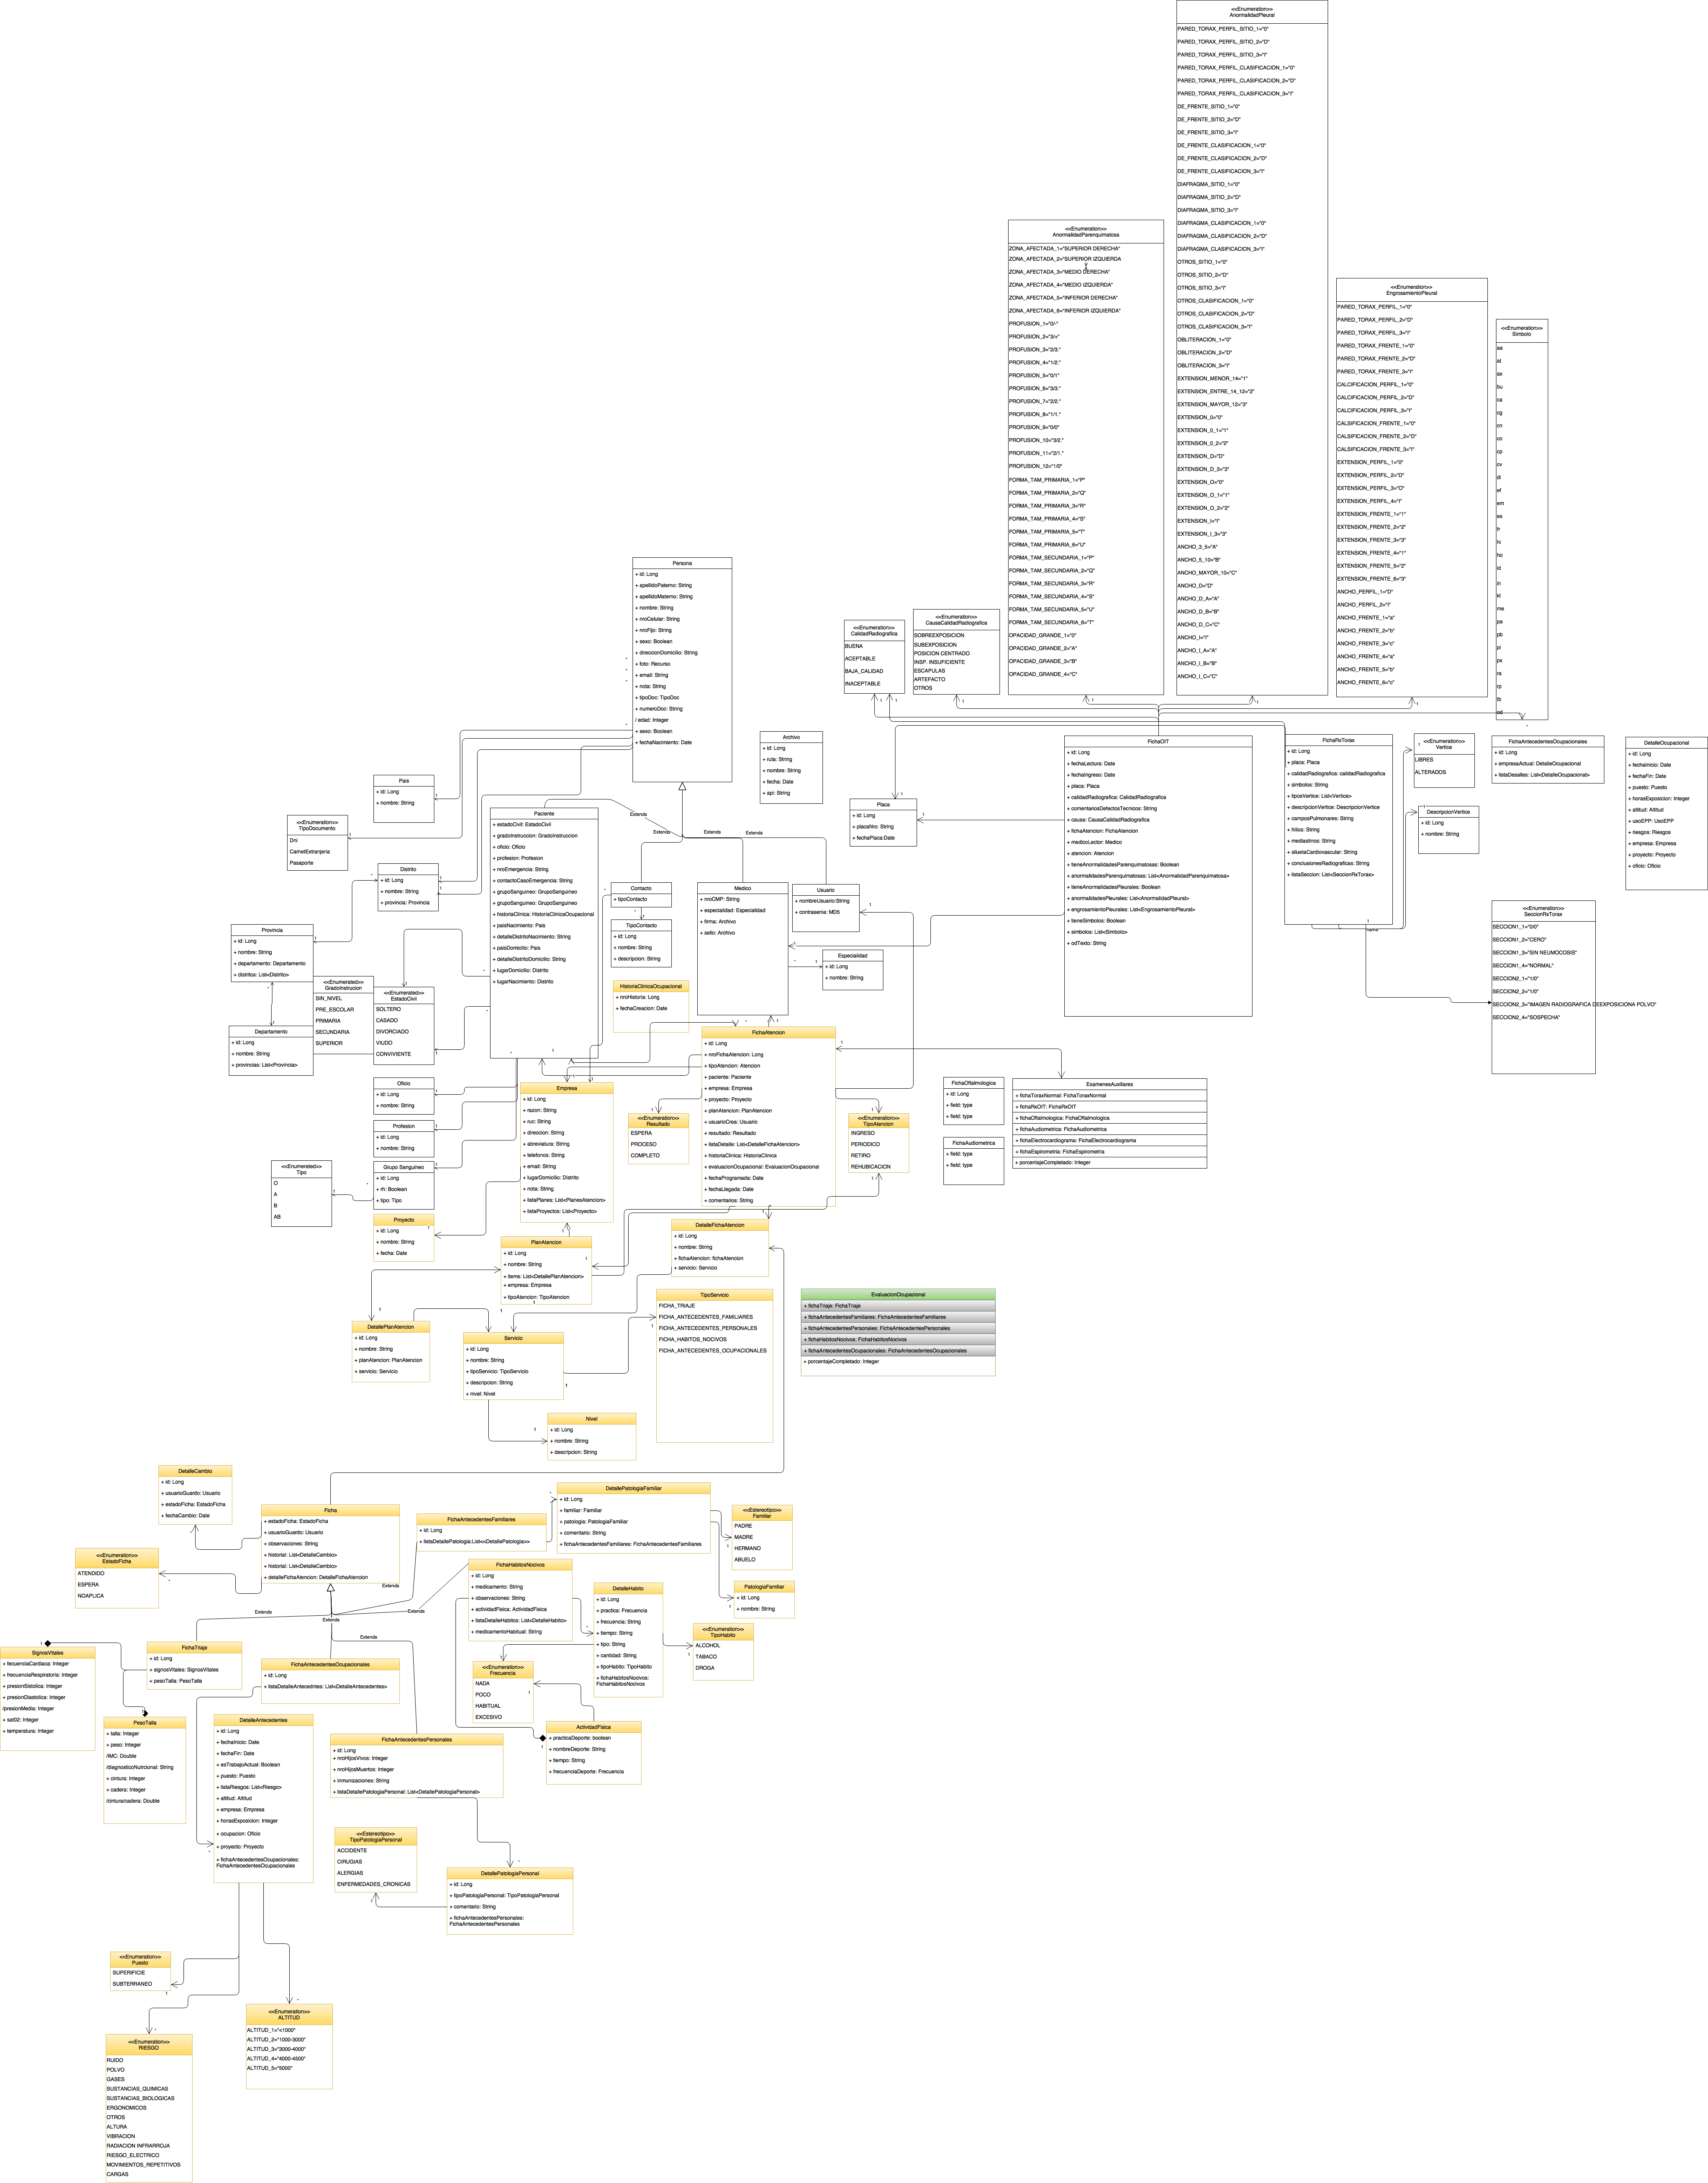
\includegraphics[width=18cm]{../imgs/disenio/DC.png}
		\caption{DC-B Diagrama de clases completo}
	\end{figure}
	\begin{figure}[H]
	    \centering
		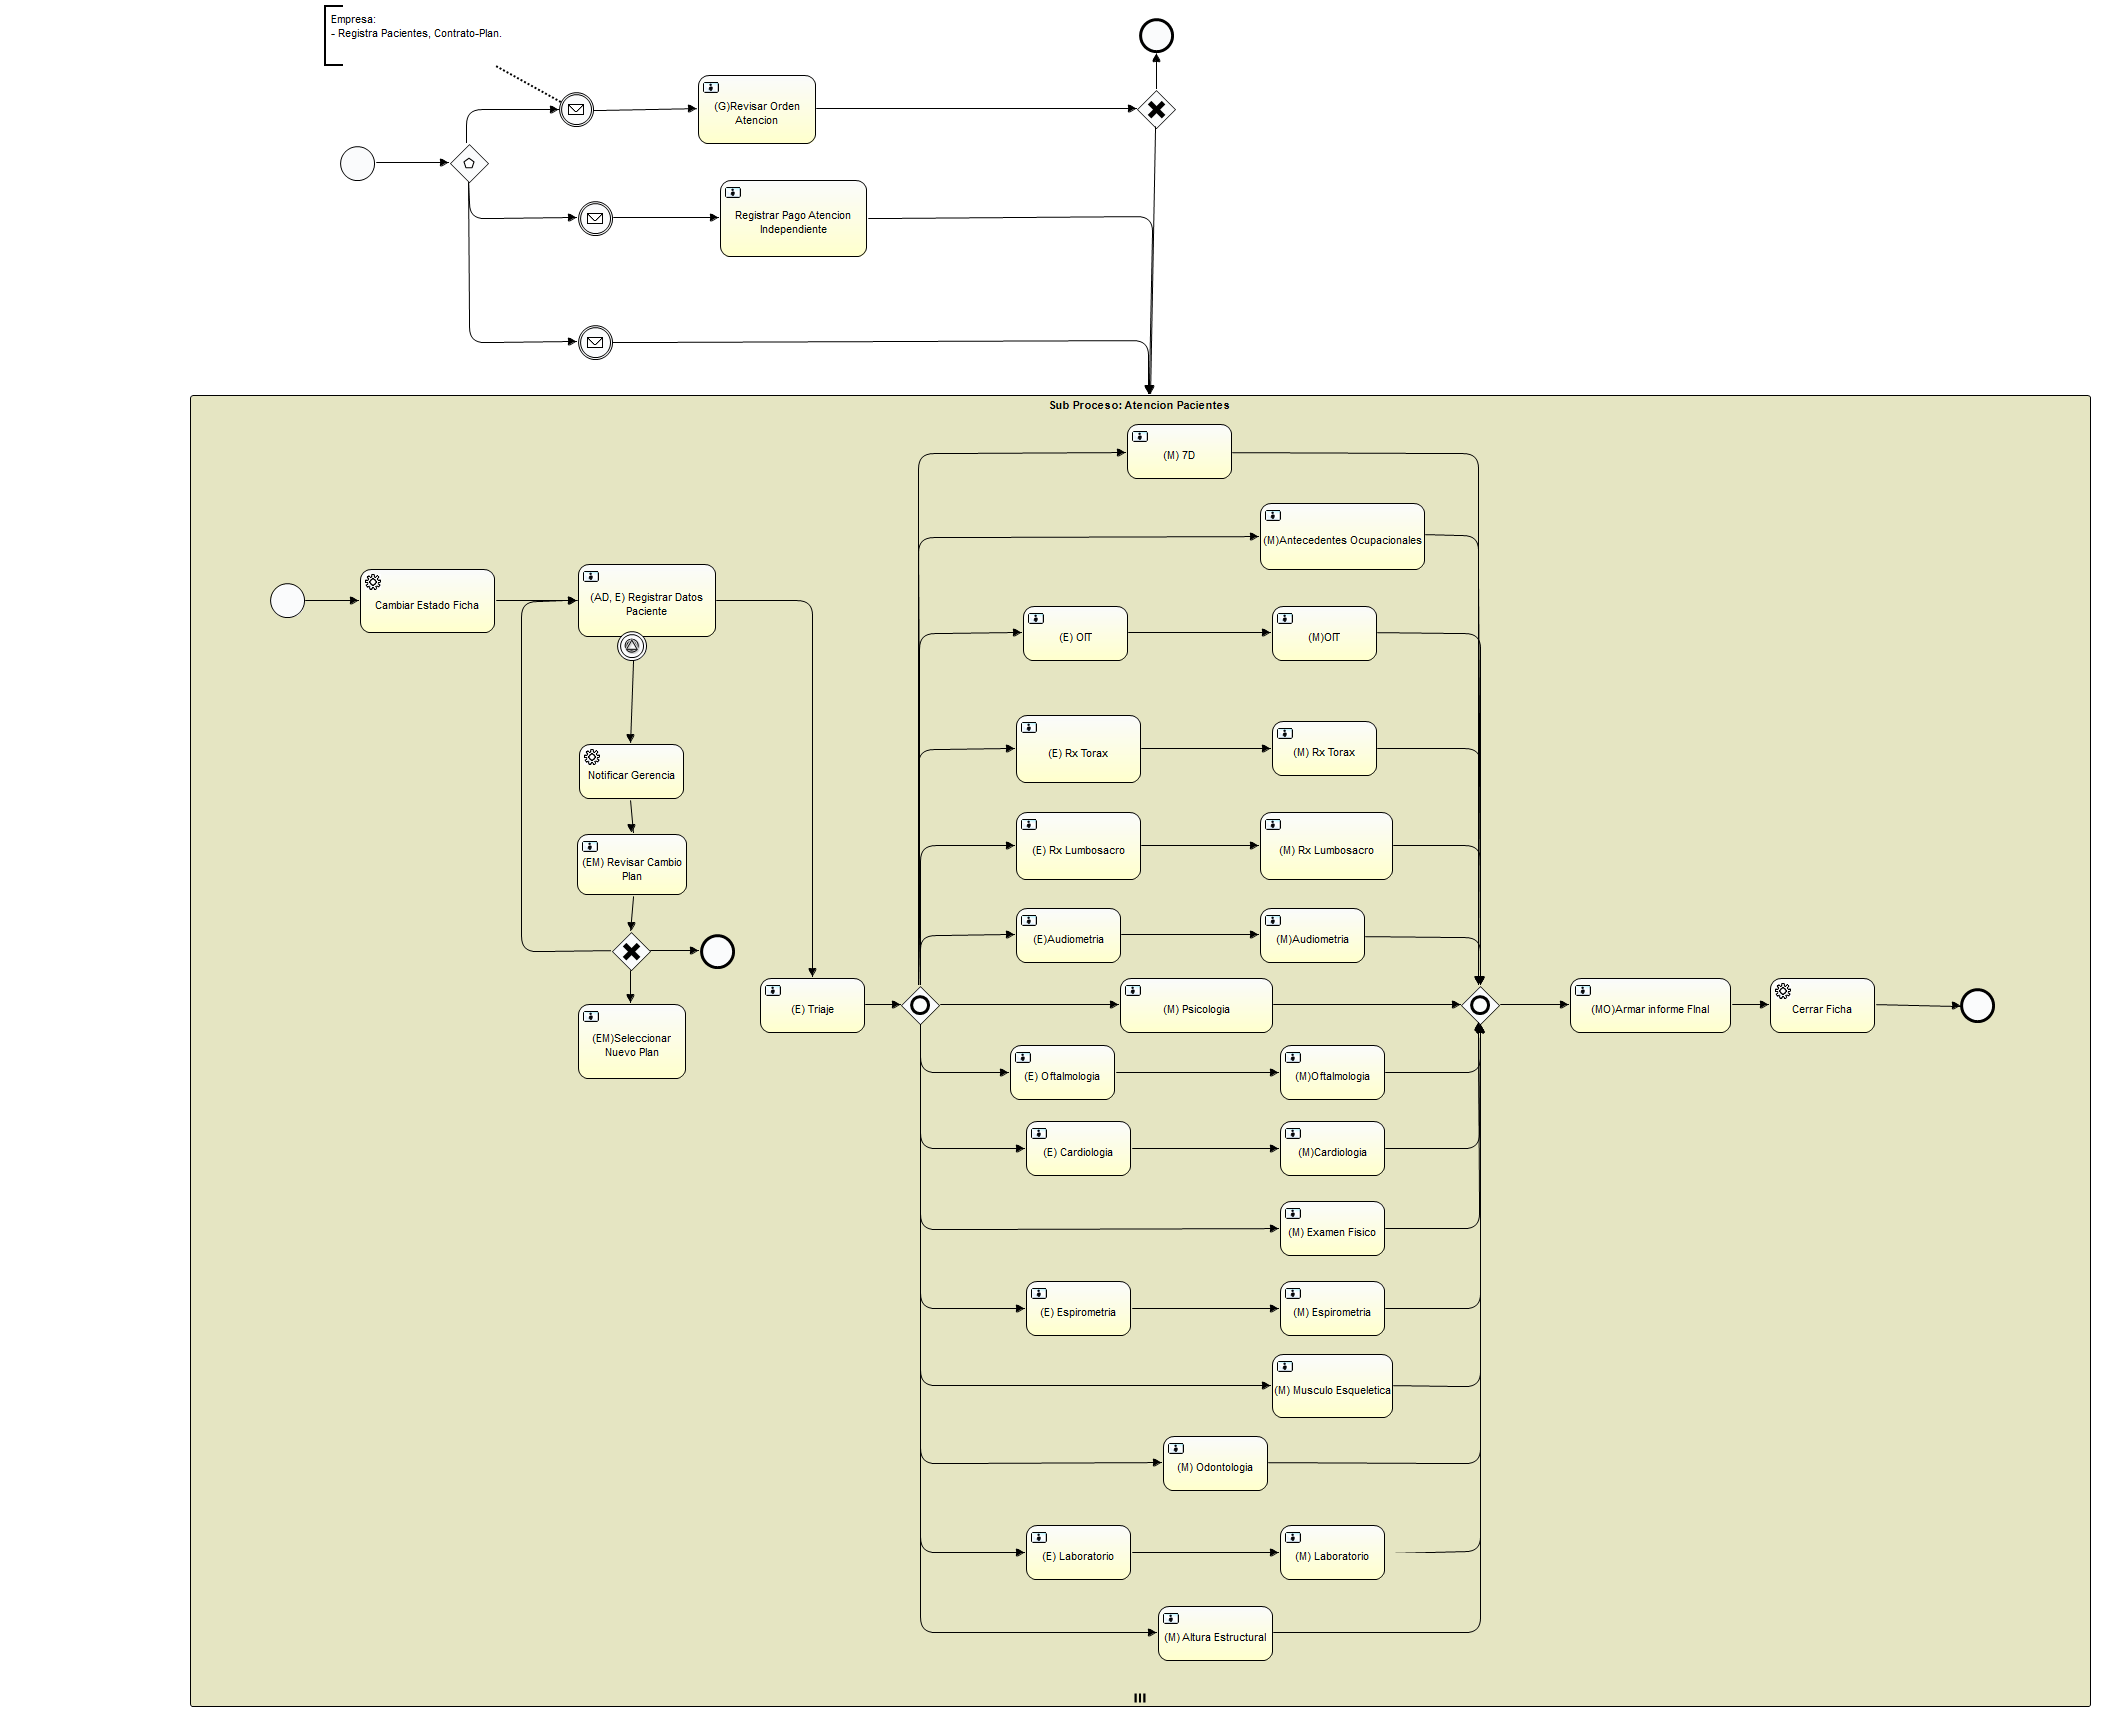
\includegraphics[width=18cm]{../imgs/disenio/ProcesoAtencion.png}
		\caption{DP-1 Diagrama BPM}
	\end{figure}
\newpage

\section{Arquitectura del Sistema}

	El Sistema sigue una arquitectura REST (Representational state trasfer) ó
	de servicios web RESTful cliente-servidor que, funciona bajo el protocolo
	HTTP, figura \ref{figure:arq1}. Básicamente el backend se encarga 
	de proporcionar recursos (previa autorización) al frontend.
	\\\
	
	\begin{figure}[ht!]
	    \centering
		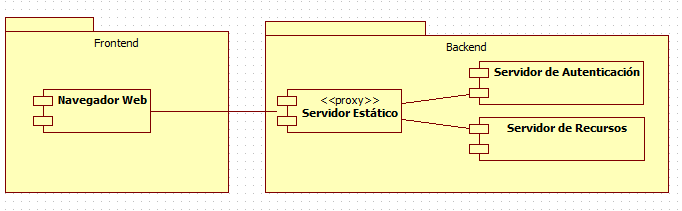
\includegraphics[width=18cm]{../imgs/disenio/arq1.png}
		\caption{DA-1 Arquitectura del Sistema}
		\label{figure:arq1}
	\end{figure}
	
	
	En la figura \ref{figure:arq2} se muestra detalladamente la interacción de los
	componentes (frontend y backend).
	\\\
	
	\begin{figure}[ht!]
	    \centering
		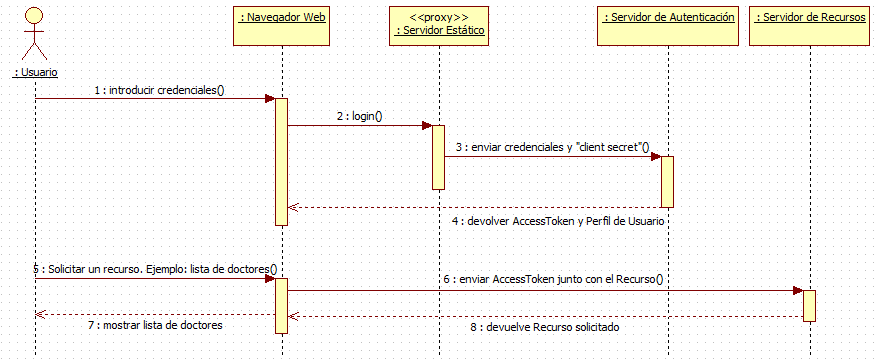
\includegraphics[width=18cm]{../imgs/disenio/arq2.png}
		\caption{DA-2 Arquitectura del Sistema (Diagrama de secuencia)}
		\label{figure:arq2}
	\end{figure}